\subsection{Schroedinger and Heisenberg picture}
\subsubsection{Schroedinger picture}
In the Schroedinger picture, we focus on the time evolution of states:
\begin{equation}  
	|\psi\rangle = |\psi\rangle(t) 
\end{equation}
In this picture we can introduce quantum circuit diagram notation, whereby:
\begin{itemize}
	\item States progress in time along horizontal parallel lines
	\item Time goes from left to right
	\item Gates denoted X,Y,Z are the pauli matrices 
		$\sigma_x,\sigma_y,\sigma_z$
	\item Gates can act on one or multiple qubits, whereby an X gate 
		on qubit 1 in a 3-qubit system should be interpreted as:
		\\$(X\otimes \mathbb{I} \otimes \mathbb{I}) (|\psi_1\rangle
		\otimes |\psi_2\rangle \otimes |\psi_3\rangle)$
\end{itemize}
\begin{figure}[h!]
	\begin{center}
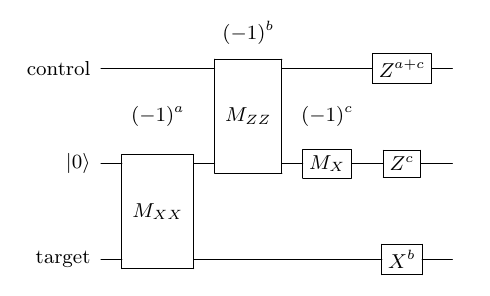
\includegraphics[scale=0.5]{img/cnotMeasureCircuit.png}\\
	\caption{A Quantum Circuit, where $|0\rangle$ is the +1
	eigenstate in $\sigma_z$-basis}
	\label{fig:circuit1}
	\end{center}
\end{figure}
\newpage

As can be seen explicitly calculated in the familiar Schroedinger 
picture in Appendix~\ref{sec:calc1}, the circuit from figure~\ref{fig:circuit1}
implements a CNOT-gate from the control qubit to the target qubit.

We will now analyze this circuit in the Heisenberg picture,
finding that it results in an equal output.

\subsubsection{Heisenberg Picture}
In this picture, we focus on the time evolution of operators instead
of states:
\begin{equation}
	A = A(t)
\end{equation}
By considering specifically the operators to which the input state
space is part of those operators eigenstatespace, we can compute
the output of any circuit:
\begin{equation}
	Circuit(|\phi\rangle) = Circuit(A)|\phi\rangle
\end{equation}
if $|\phi\rangle$ is an eigenstate of A.\\
We call an operator/gate, to which an input state is an eigenvector the 
``Stabilizer'' of that input state. \\
The ``Stabilizer group'' is a group of such operators, comprising the
Stabilizers that stabilize all allowed input states \\
So e.g.\ the input state in figure~\ref{fig:circuit1} is only 
stabilized by $\mathbb{I} \otimes Z \otimes \mathbb{I}$ 
(and trivially $\mathbb{I} \otimes \mathbb{I} \otimes \mathbb{I}$).\\
Given a Measurement M and a density matrix $\rho$, after the Measurement
$\rho\rightarrow\rho'$ with:
\begin{equation}
	\rho'=\frac{M\rho M^{\dag}}{tr(M\rho M^{\dag})}
\end{equation}
So in our case, if the measurement result is +1 after the first Measurement,
to obtain the ``heisenberg-state'' we need to compute:
\begin{equation}
	\frac{(\mathbb{I}\otimes\mathbb{I}\otimes\mathbb{I}+
	\mathbb{I}\otimes X \otimes X) \mathbb{I} \otimes Z \otimes \mathbb{I}
	(\mathbb{I}\otimes\mathbb{I}\otimes\mathbb{I}+
	\mathbb{I}\otimes X \otimes X)^{\dag}}{tr((\mathbb{I}\otimes\mathbb{I}\otimes\mathbb{I}+
	\mathbb{I}\otimes X \otimes X) \mathbb{I} \otimes Z \otimes \mathbb{I}
	(\mathbb{I}\otimes\mathbb{I}\otimes\mathbb{I}+
	\mathbb{I}\otimes X \otimes X)^{\dag})}
\end{equation}












